\section{Closed-Loop Optimisation Method}
\label{ch1:sec:closed-loop-optimisation-method}

In the previous two sections, the key network parameters and associated cost functions have been established.
Then the used network models, data and battery models were explained.
Now, the implemented method on generating a traditional ESMU schedules is presented, before presenting the novel approach of adjusting this schedule using on-line readings.

\subsection{ESMU Schedule generation}
\label{ch1:subsec:esmu-schedule-generation}

As discussed in the literature review in Chapter \ref{ch-review}, the main goals when scheduling battery operation are to achieve ``valley-filling'' and ``peak-shaving'' behaviour.
It has been identified, that both the Peak-to-Average Ratio (PAR) as well as the min-max-difference (MMD) are good indicators of how well the pursued behaviours have been implemented.
Therefore, a half-hourly PAR scheduling cost, $\zeta^*_{PAR}(\textbf{s}^*_{ESMU}, \textbf{s}^*_{network\;\;load})$, and a half-hourly MMD scheduling cost, $\zeta^*_{MMD}(\textbf{s}^*_{ESMU}, \textbf{s}^*_{network\;\;load})$, are defined as follows:

\begin{equation}
\begin{split}
	\zeta_{PAR}(\textbf{s}_{A}, \textbf{s}_{B}) :=& \frac{\max_k \left| \textbf{s}_{A}+\textbf{s}_{B}\right|}{\frac{1}{K}\sum_{k=1}^{K}\left[{s}_{A}(k)+{s}_{B}(k)\right]} - 1\\
	& \text{where } {s}_{A}(k) \in \textbf{s}_{A} \text{ and } {s}_{B}(tk \in \textbf{s}_{B}
\end{split}
\label{ch1:equ:peak-to-average-definition}
\end{equation}

\begin{equation}
	\zeta_\text{MMD}(\textbf{s}) := \frac{\max_k \left(\textbf{s}\right) - \min_k\left(\textbf{s}\right)}{\frac{1}{K}\sum_{t=1}^{\frac{T_\text{sch}}{K}}s(t)}
	\text{ where } (s(t)) = \textbf{s}
\label{ch1:equ:min-max-difference-definition}
\end{equation}

Both costs are functions of the entire half-hourly ESMU schedule, $\textbf{s}^*_{ESMU}$, and the entire half-hourly network load profile, $\textbf{s}^*_{network\;\;load}$, where only the ESMU schedule is adjustable by an optimisation algorithm.
For this piece of work, a Sequential Quadratic Programming (SQP) approach was chosen to solve the following minimisation problem.
Reasons behind this choice are the SQP's robustness and speed, since it is built on the well established Newton-Raphson Method, as well as its ability to cope with nonlinear constraints.
It is this latter point that is most important, since the battery model's solving constraints are inherently nonlinear; the Newton-Raphson Method by itself is unable to solve with this kind of nonlinear constraints.
The final minimisation problem that was passe into the SQP solver can be formulated as:

\begin{equation}
\begin{split}
	\min_{\textbf{s}^*_\text{ESMU}} & \left\{\zeta_\text{PAR}(\textbf{s}^*_\text{ESMU}, \textbf{s}^*_\text{net}) + \zeta_\text{MMD}(\textbf{s}^*_\text{ESMU}, \textbf{s}^*_\text{net}) + \zeta_\text{TRA}(\textbf{s}^*_\text{ESMU}, \textbf{s}^*_\text{net})\right\}\\
	\text{s.t. }& \begin{cases}
		p_\text{bat}(t) \leq C_f\times C_\text{bat}\\
		\left|s_{\text{ESMU},\phi}(t)\right| \leq S_\text{rating} \forall \phi\\
		0 \leq SOC(t) \leq 1
	\end{cases}
\end{split}
\label{ch1:equ:scheduling-cost}
\end{equation}

To summarise, this minimisation therefore minimises two costs by adjusting the half-hourly ESMU schedule, $\textbf{s}^*_{ESMU}$, given a certain half-hourly network load (or forecast) $\textbf{s}^*_{network\;\;load}$.
These two costs both capture the PAR and MMD of the resulting power profile, and when minimised to zero, indicate a perfectly flat power curve.
The minimisation is constrained to not exceed the battery's maximum charge/discharge rate (i.e. $s_{battery}(t) \leq C_{factor} \times C_{battery} \forall t$), to not exceed the PMU's phase power rating (i.e. $\left|s_{ESMU,p}(t)\right| \leq S_{rating} \forall p \forall t$), and to not over- or under-charge the battery (i.e. $0 \leq SOC(t) \leq 1 \forall t$).

For the work presented in this chapter, the supplied half-hourly network load (or forecast) was extrapolated from sub-half-hourly data.
This forecast can be seen as if it had been generated with perfect foresight.
Doing this does not skew the already imperfect performance that would be obtained when applying the half-hourly schedule.
Therefore, any additional improvement or worsening is the result of the sub-half-hourly schedule adjustments.

In the following figure, a visualisation is provided where the impact of this half-hourly ESMU schedule becomes apparent.

\begin{figure}\centering
	\subfloat[Half-hourly ESMU power impact ($\Delta S = 9.46kW$)]{%
		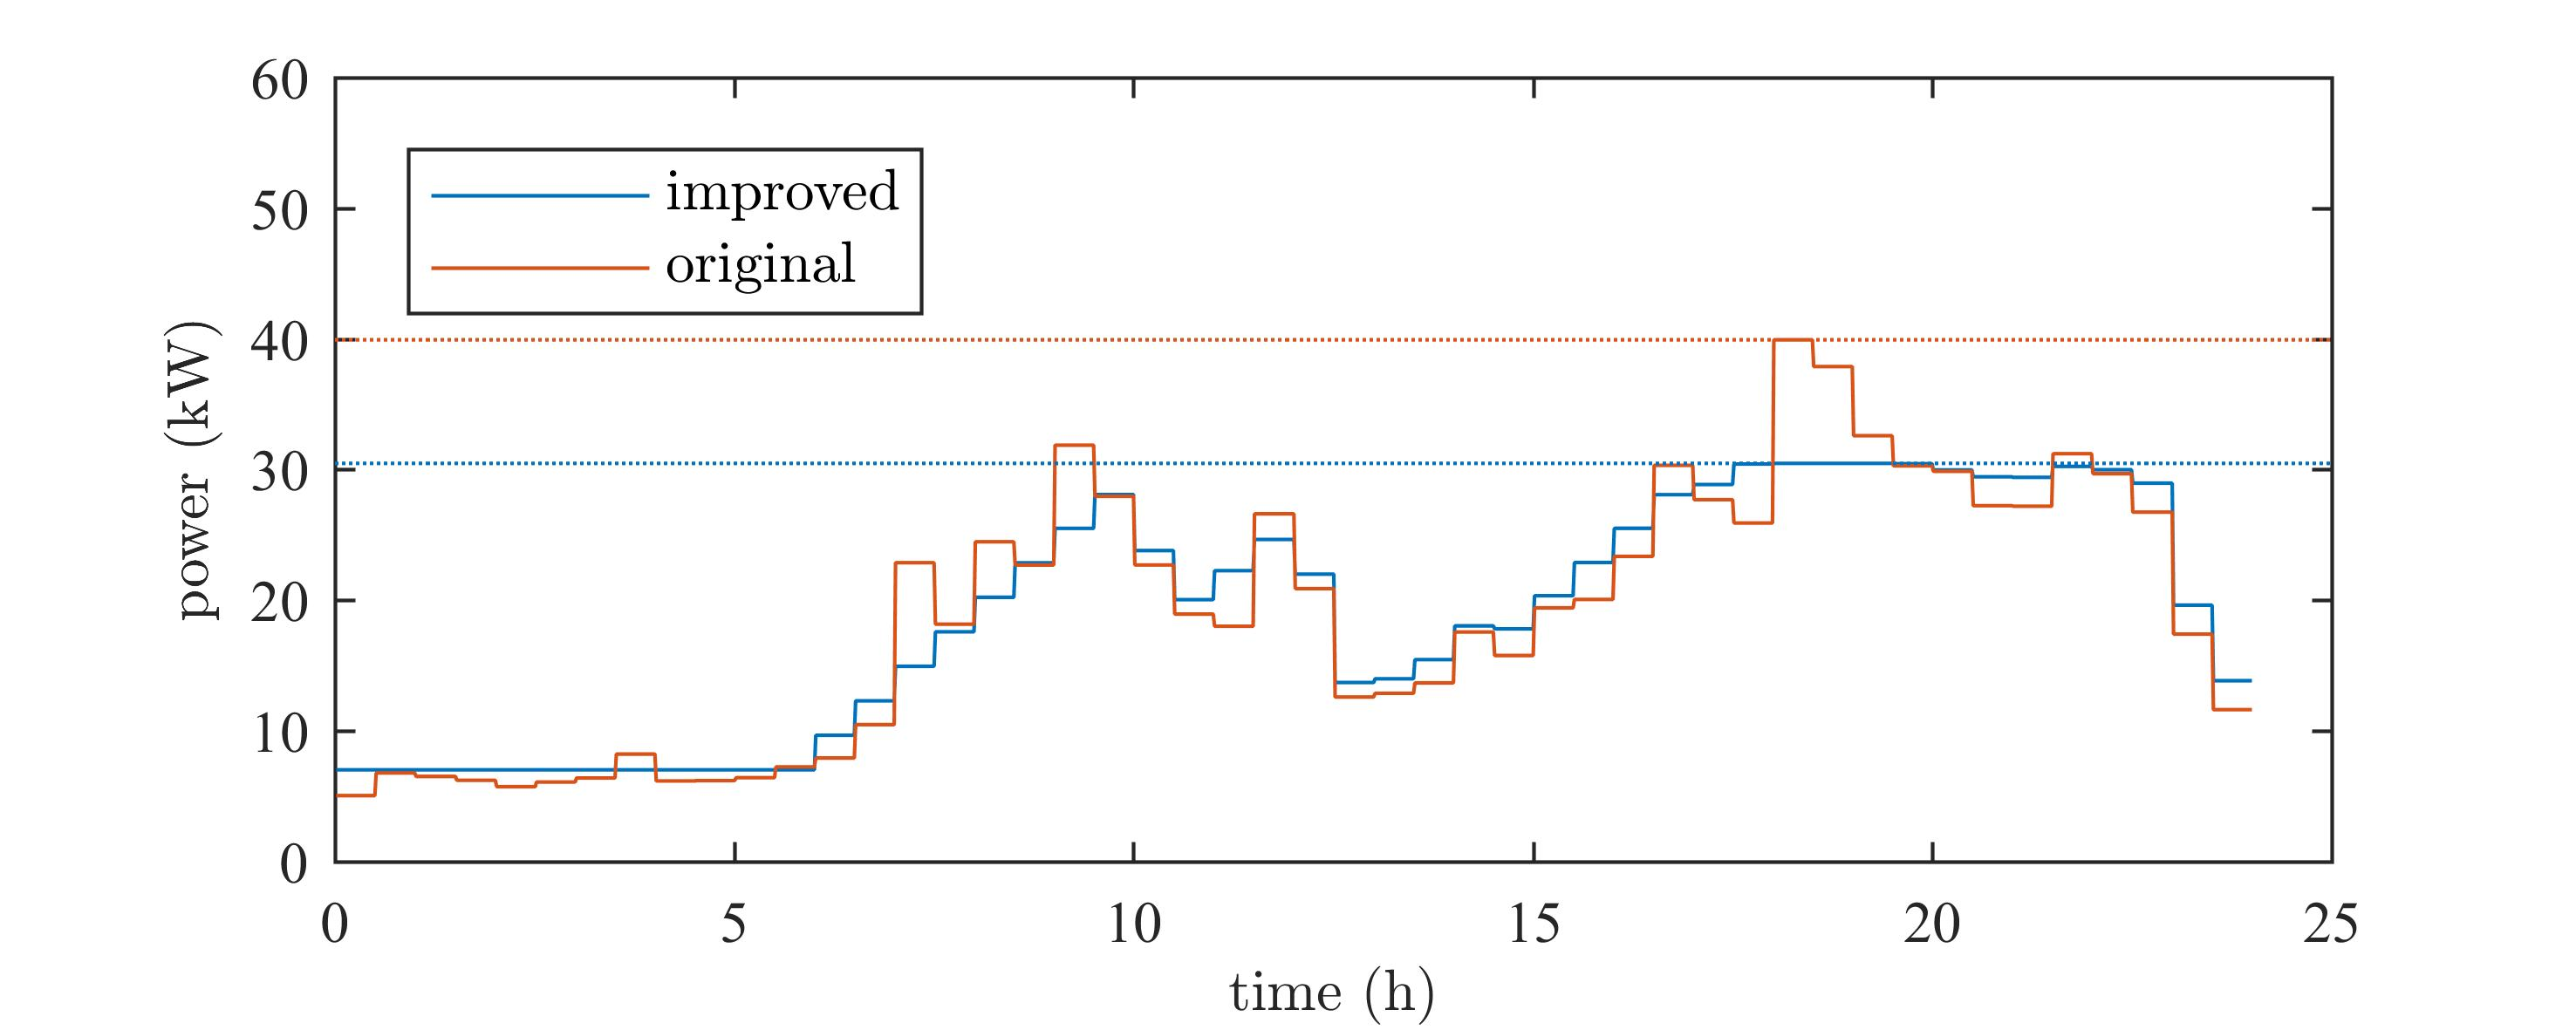
\includegraphics{_chapter1/fig/improved-half-hourly-network-power}%
		\label{ch1:subfig:improved-half-hourly-network-power}%
	}
	\vspace{5mm}
	\subfloat[Sub-half-hourly ESMU power impact ($\Delta S = 6.36kW$)]{%
		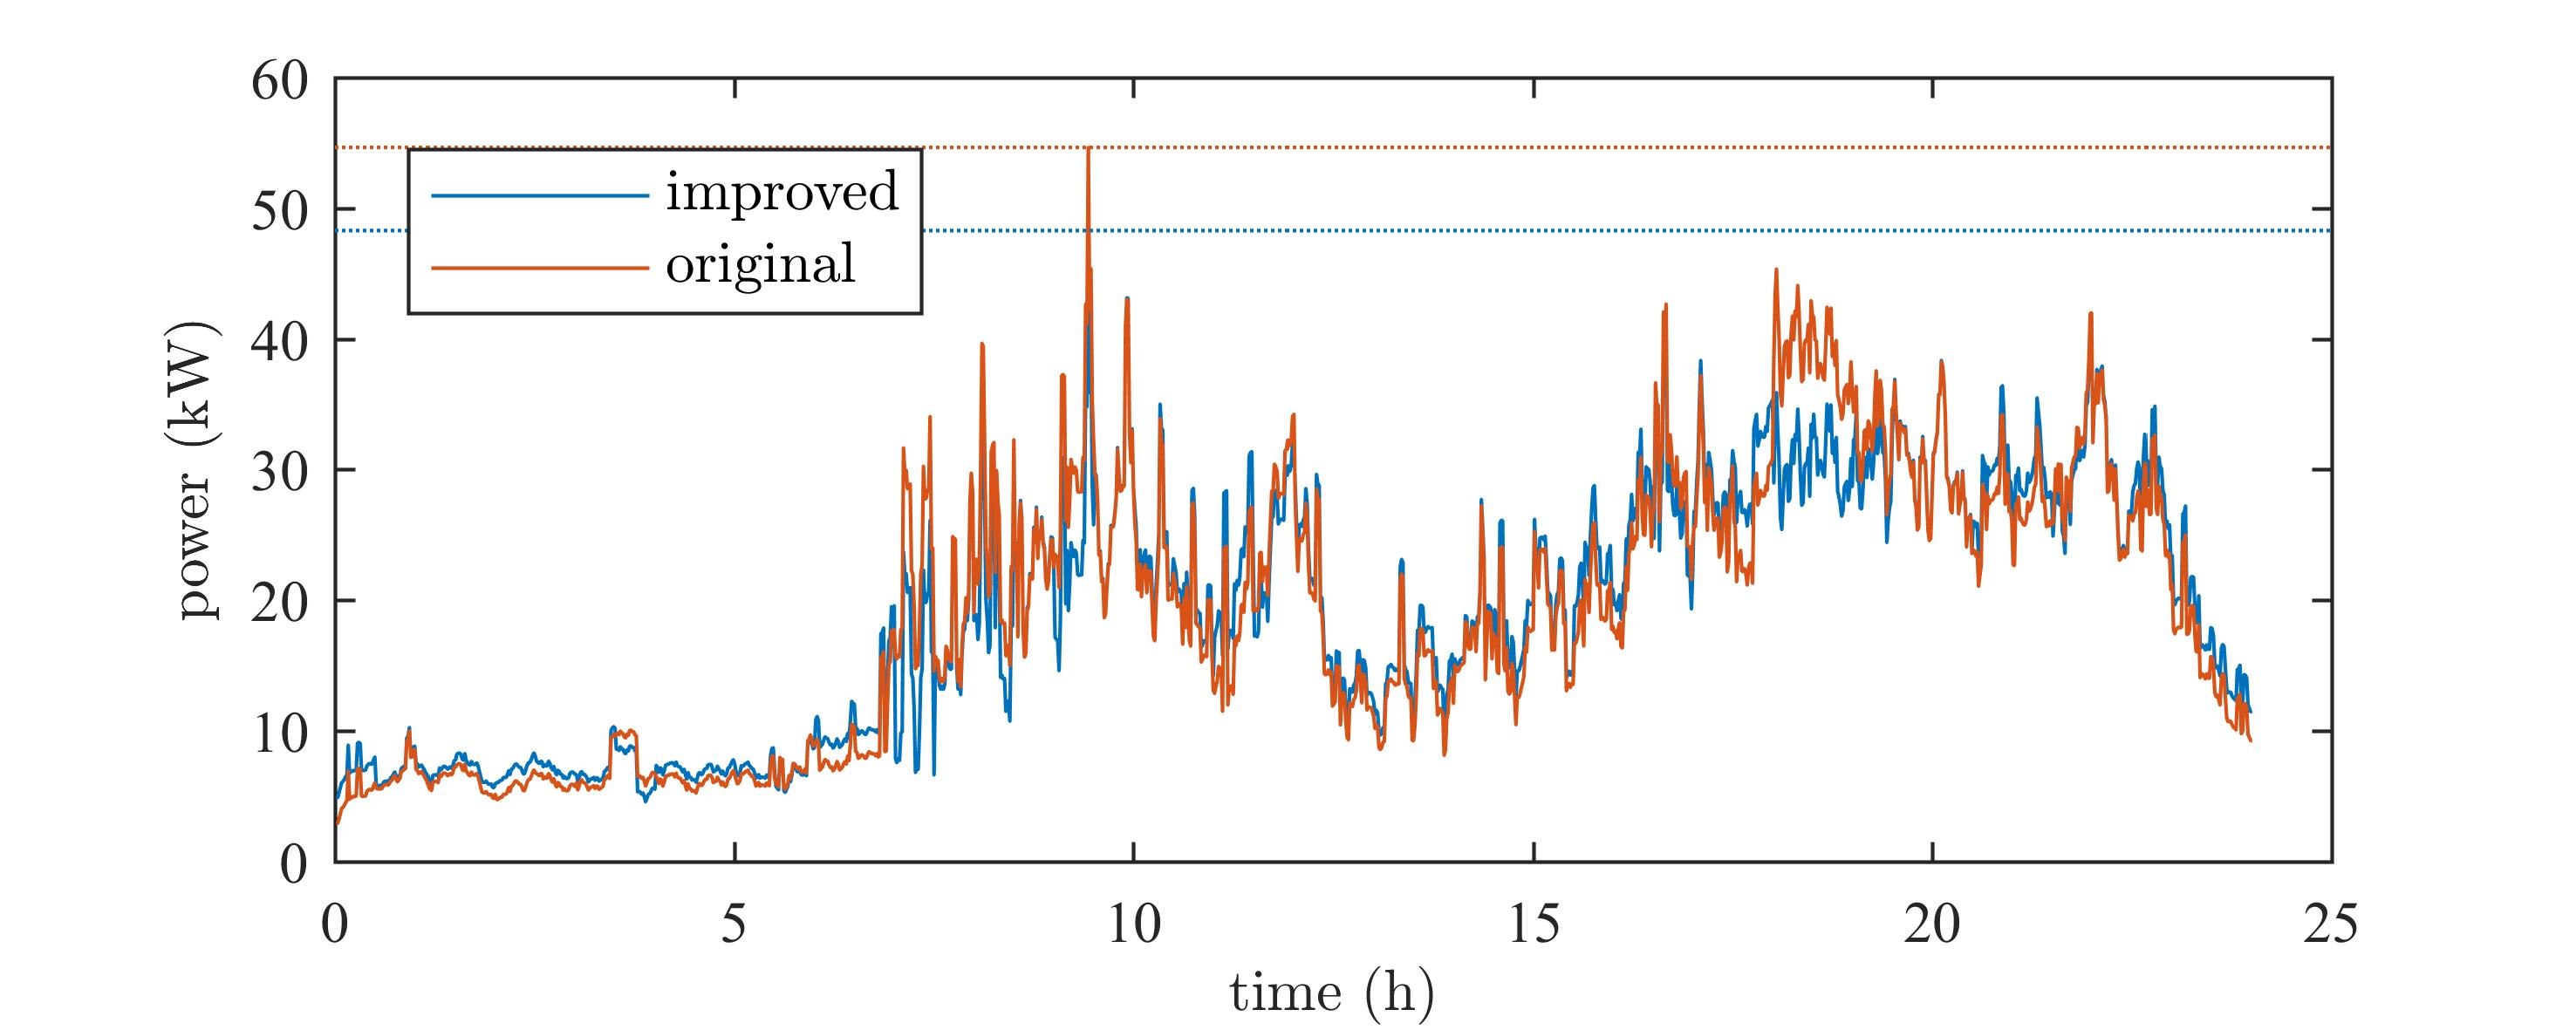
\includegraphics{_chapter1/fig/improved-sub-half-hourly-network-power}%
		\label{ch1:subfig:improved-sub-half-hourly-network-power}%
	}
	\caption{Impact of half-hourly ESMU schedule on sub-half-hourly power profile}
	\label{ch1:fig:improved-network-power}
\end{figure}

It can be seen that the half-hourly profile in Figure \ref{ch1:subfig:improved-half-hourly-network-power} is dominated by an evening peak in demand.
However, the actual demand, as it is plotted in Figure \ref{ch1:subfig:improved-sub-half-hourly-network-power}, has a much larger demand spike during the morning hours, which is addressed not as strongly as the evening peak.
Therefore, the compared peak power shaving dropped from 9.46kW to only 6.36kW, although only 50\% of the battery's discharge capacity is used.
Nonetheless, the overall improvement yielded by the ESMU schedule is still noticeable (given that it was scheduled using perfect half-hourly foresight). 

In the following section, the underlying closed-loop schedule adjustment method is explained, where it will be shown how individual key network operation can be positively impacted without deviating from this already optimised half-hourly schedule.
The constraint of having to follow this half-hourly ESMU schedule is lifted in Chapter \ref{ch2}, where a real-time schedule adjustment method is proposed and researched.

\subsection{Closed-Loop Schedule Adjustment Method}

From all cost functions defined in Section \ref{ch1:sec:key-network-parameters}, a weighted sum of all costs was generated:

\begin{multline}
	\zeta(\textbf{v}_\text{ss}(t), \textbf{v}_\text{ESMU}(t), \textbf{v}_{\text{load}}(t), \textbf{s}_{ss}(t), \textbf{i}_{ss}(t), \textbf{i}_{\text{line}}(t), s_\text{losses}(t), \boldsymbol{\alpha}) :=\\
	\alpha_1 \sum_{\phi=1}^\Phi\zeta_\text{voltage}(v_{\text{ss},\phi}(t))%\\
	+ \alpha_2 \sum_{\phi=1}^\Phi\zeta_\text{voltage}(v_{\text{ESMU},\phi}(t))%\\
	+ \alpha_3 \zeta_\text{\text{load} voltage}(\textbf{v}_{\text{load}}(t))\\
	+ \alpha_4 \zeta_\text{unbalance}(\textbf{s}_{ss}(t))%\\
	+ \alpha_5 \zeta_\text{PF}(\textbf{s}_{ss}(t))%\\
	+ \alpha_6 \zeta_{\text{neutral load}}(\textbf{s}_{ss}(t))\\
	+ \alpha_7 \zeta_\text{fuse utilisation}(\textbf{i}_{ss}(t))%\\
	+ \alpha_8 \zeta_\text{\text{line} utilisation}(\textbf{i}_{\text{line}}(t))%\\
	+ \alpha_9 \zeta_\text{losses}(s_\text{losses}(t)) \\
	 \text{where } \phi \in \{1, \dots, \Phi\} \text{ and } \Phi \in \mathbb{Z}_{>0} \text{ and } \boldsymbol{\alpha} = \{\alpha_1, \dots, \alpha_9\}
\label{ch1:equ:weighted-sum-cost-function}
\end{multline}
